\chapter{流量检测系统的设计与实现}
\section{引言}
本文实现的流量异常检测系统按照功能需求可以分为三个模块:数据采集和分析模块,异常检测模块,终端预警模块。
TODO: 图中加入关系矩阵
\begin{figure}
    \centering
    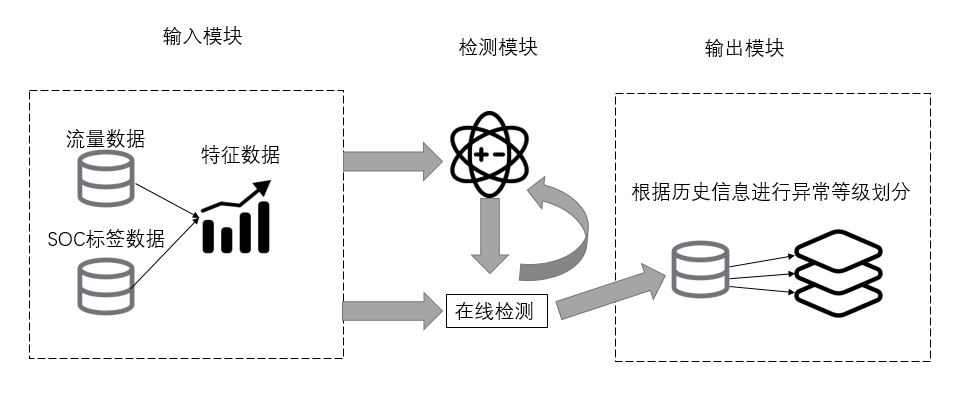
\includegraphics[scale=0.6]{系统架构图.png}
    % 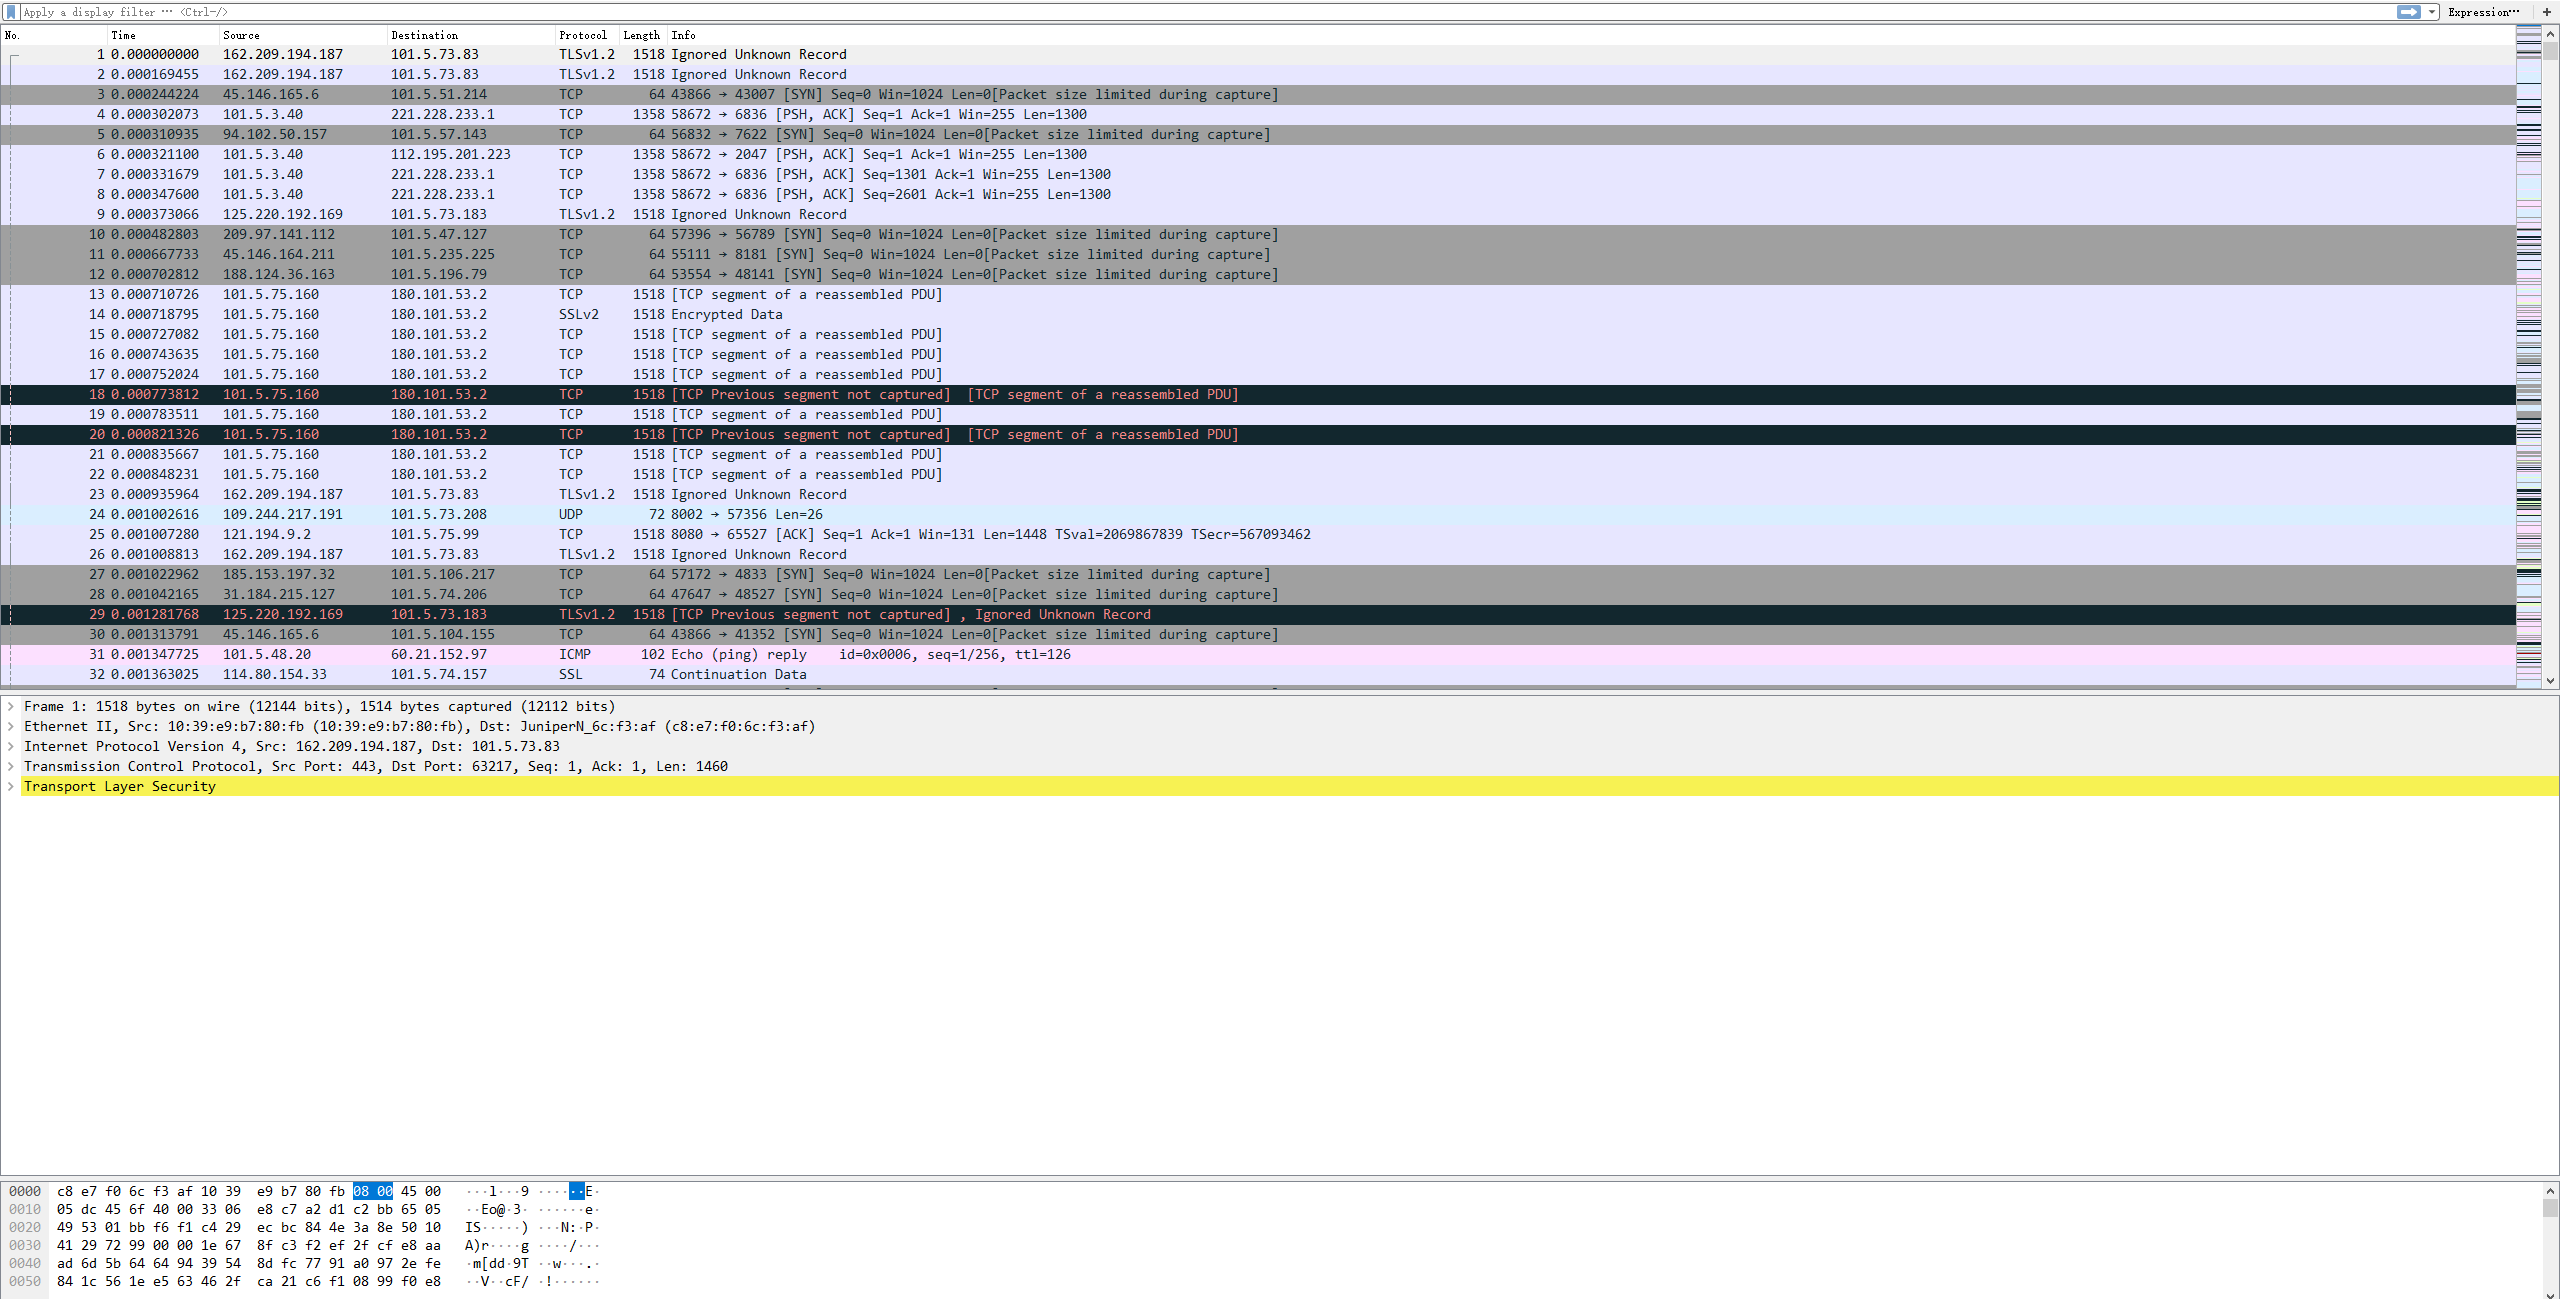
\includegraphics[width=0.6\linewidth]{wireshark流量图.png}
    \caption{系统架构图}
    \label{fig:arch}
  \end{figure}


下面是对各个模块的介绍:

待补充。

% \section{使用大数据平台应对大规模流量的必要性}
\section{spark 平台介绍}
Apache Spark是由UC Berkeley AMP Lab开源的用于大规模数据处理的统一分析引擎\cite{spark},现如今已经成为Apache软件基金会的顶级开源项目。Spark原理与Hadoop类似,都是基于MapReduce进行分布式计算,但是功能更加丰富,且支持SQL查询、流式处理、图计算等功能。
% 它基于Hadoop MapReduce,并且扩展了MapReduce模型以有效地将其用于更多类型的计算,其中包括交互式查询和流处理。
% Spark能比Hadoop运算更快的主要原因在于:Hadoop 在进行一次MapReduce 运算之后,会将数据的运算结果从内存写入到磁盘中,第二次MapReduce运算时再从磁盘中读取数据,通过两次对磁盘的操作,会增加多余的IO消耗;对比来看,Spark则是将数据一直缓存在内存中,运算时直接从内存读取数据,只有在必要时,才将部分数据写入到磁盘中。
Spark具有以下几个特点:

\begin{itemize}
  \item 速度快,Spark的速度比Hadoop要快100倍以上,图\ref{fig:Logistic regression in Hadoop and Spark}是一项逻辑回归任务在Hadoop和Spark两个系统的运行时长对比。这是因为Spark基于内存计算,而Hadoop MapReduce必须进行读取和写入磁盘,IO操作比内存操作更加耗时。
  % 另外,Spark中引入
  % 使用最先进的 DAG(Directed Acyclic Graph,有向无环图)调度程序、查询优化器和物理执行引擎,在处理批量处理以及处理流数据时,具有较高的性能。
  \item 易用性。Spark提供了80余种高级API,可以轻松编写高度并行的应用程序。Spark支持Java, Scala, Python, R, and SQL等多种编程语言。
  \item 兼容性。Spark可以运行在Hadoop模式、Mesos模式、Standalone独立模式或Cloud中,并且还可以访问各种数据源,包括本地文件系统、HDFS、Cassandra、HBase和Hive等。
\end{itemize}
\begin{figure}
  \centering
  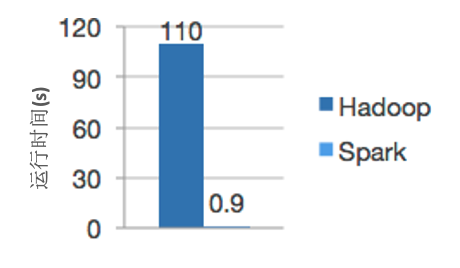
\includegraphics[width=0.3\linewidth]{logistic-regression.png}
  \caption{Logistic regression in Hadoop and Spark}
  \label{fig:Logistic regression in Hadoop and Spark}
\end{figure}


如图\ref{fig:Spark组件}所示,Spark项目包含多个独立组件。其最核心的模块为深蓝色的Spark Core,其定义了核心API,如弹性分布式数据集(Resilient Distributed Datasets,RDD),该模块也负责调度、监控计算集群中的计算任务,具有内存管理,故障恢复,与管理系统、存储系统交互等功能。为了满足分布式计算系统的可扩展性,Spark支持在各种集群管理器之上运行,例如图中灰色的模块Hadoop YARN,Apache Mesos以及浅蓝色的Spark自身的“独立调度程序”(Standalone Scheduler)。在Spark Core之上,具有四个组件:Spark SQL、Spark Streaming、MLlib、GraphX。本文中的系统主要使用Spark Streaming组件。


% 从本质上讲,Spark是一个“计算引擎”,负责调度,分发和监视由跨许多工作机或计算集群的许多计算任务组成的应用程序。Spark Core包含Spark的基本功能,包括任务计划,内存管理,故障恢复,与存储系统交互等功能。 Spark Core中也定义了核心API,如弹性分布式数据集(Resilient Distributed Datasets,RDD)。 在后台,Spark需要从一个计算节点有效地扩展到成千上万个计算节点。 为了在实现最大灵活性的同时实现此目的,Spark支持在各种集群管理器之上运行,包括Hadoop YARN,Apache Mesos和Spark本身包含的称为“独立调度程序”(Standalone Scheduler)的简单集群管理器。 在Spark Core之上,具有四个组件:Spark SQL、Spark Streaming、MLlib、GraphX。本文中的系统主要使用Spark Streaming组件。

\begin{figure}
  \centering
  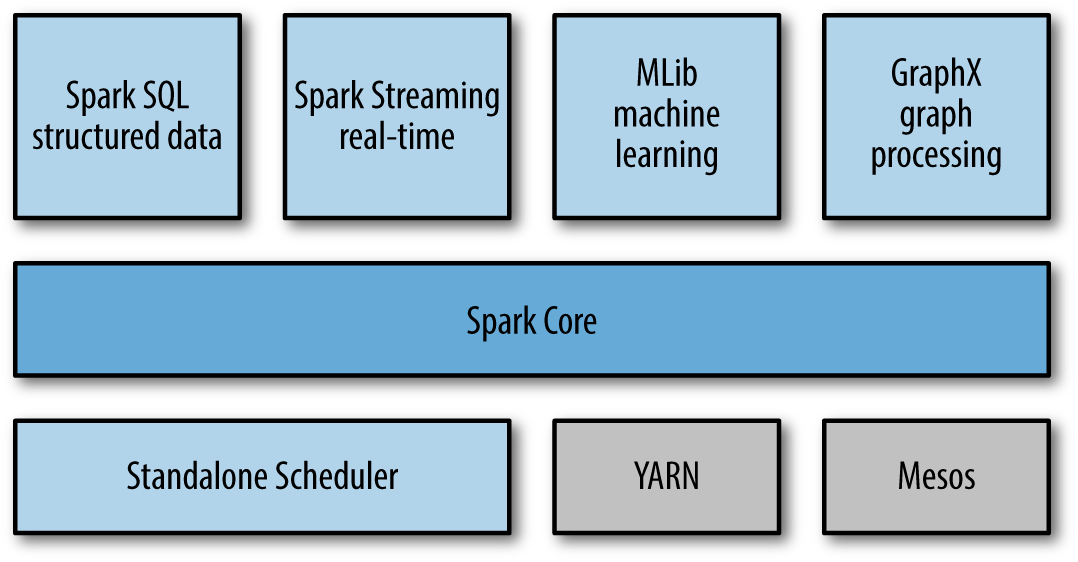
\includegraphics[width=0.6\linewidth]{spark-stack.png}
  \caption{Spark组件}
  \label{fig:Spark组件}
\end{figure}
% Spark Core是 Spark 的核心,主要负责任务调度等管理功能。Spark
% Core 的实现依赖于 RDDs(Resilient Distributed Datasets,
% 弹性分布式数据集)的程序抽象概念。

% Spark Streaming这个模块的作用主要是处理流数据,支持流数据的可伸缩和容错处理,可以与 Flume(针对数据日志进行优化的一个系统)和 Kafka(针对分布式消息传递进行优化的流处理平台)等已建立的数据源集成。Spark Streaming 的实现,也需要通过 RDD的抽象概念,使其在为流数据(如批量历史日志数据)编写应用程序时,能够更灵活,也更容易实现。

% Spark 具有多种运行模式,包括本地运行模式(Local 模式)、独立运行模式(Standalone 模式)、Mesos、YARN(Yet Another Resource Negotiator)、Kubernetes 模式等。本地运行模式是 Spark 的众多模式中最简单的一种,也可称作伪分布式模式。本文实验中所使用的系统模式即为本地运行模式。至于独立运行模式,它是 Spark 自带的一种集群管理模式,而Mesos 及 YARN 两种模式也都是较常使用的集群管理模式。它们的差别是,独立运行模式相对于Mesos 及 YARN 两种集群运行模式而言,又更为简单,且容易部署。


% 至于分布式部署模式,Spark 也有多种选择,而主要支持的三种部署模式分别是:Standalone、Spark on YARN和 Spark on Mesos模式。首先,Standalone模式为 Spark 自带的一种集群管理模式,即独立模式,自带完整的服务,可单独部署到一个集群中,无需依赖任何其他资源管理系统。我们知道,Standalone模式是最简易,同时也是最方便部署的一种模式。此模式是 Spark 实现的资源调度框架,其主要的节点包括有Driver 节点、Master 节点以及 Worker 节点。其次,Spark on YARN模式,是 Spark 运行在Hadoop YARN框架之上的一种模式。Hadoop YARN(Yet Another Resource Negotiator,另一种资源协调者)是一种新的 Hadoop 资源管理器,它是一个通用资源管理系统,可为上层应用提供统一的资源管理和调度。最后,Spark on Mesos模式,是 Spark 运行在Apache Mesos框架之上的一种模式。Apache Mesos是一个更强大的分布式资源管理框架,负责集群资源的分配,它允许多种不同的框架部署在其上,包括YARN。同时,它也被称为是分布式系统的内核。

% Spark 底层还支持多种数据源,能够从其它文件系统读取数据,如 HDFS、Amazon S3、Hypertable、HBase 等。Spark 对这些文件系统的支持,同时也丰富了整个 Spark 生态的运行环境。

% Spark 支持多种分布式部署模式,主要支持三种部署模式,分别是:Standalone、Spark on YARN和 Spark on Mesos模式。

% Standalone模式为 Spark 自带的一种集群管理模式,即独立模式,自带完整的服务,可单独部署到一个集群中,无需依赖任何其他资源管理系统。它是 Spark 实现的资源调度框架,其主要的节点有 Driver 节点、Master 节点和 Worker 节点。Standalone模式也是最简单最容易部署的一种模式。

% Spark on YARN模式,即 Spark 运行在Hadoop YARN框架之上的一种模式。Hadoop YARN(Yet Another Resource
% Negotiator,另一种资源协调者)是一种新的 Hadoop 资源管理器,它是一个通用资源管理系统,可为上层应用提供统一的资源管理和调度。

% Spark on Mesos模式,即 Spark 运行在Apache Mesos框架之上的一种模式。Apache Mesos是一个更强大的分布式资源管理框架,负责集群资源的分配,它允许多种不同的框架部署在其上,包括YARN。它被称为是分布式系统的内核。

% 三种架构都采用了Master/Worker(Slave)的架构,Spark 分布式运行架构大致如下:
% \begin{figure}
%     \centering
%     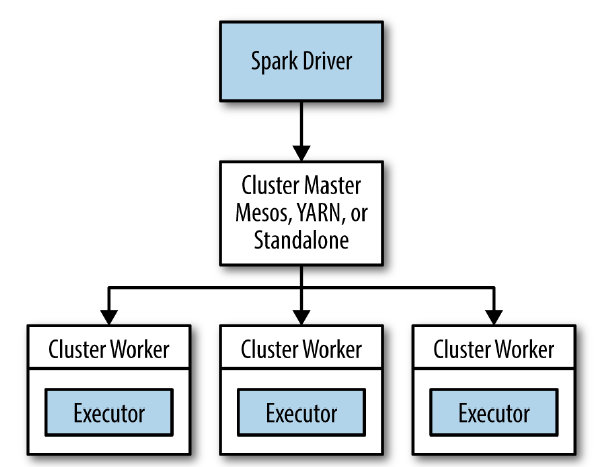
\includegraphics[scale=0.6]{spark分布式运行架构.jpg}
%     % 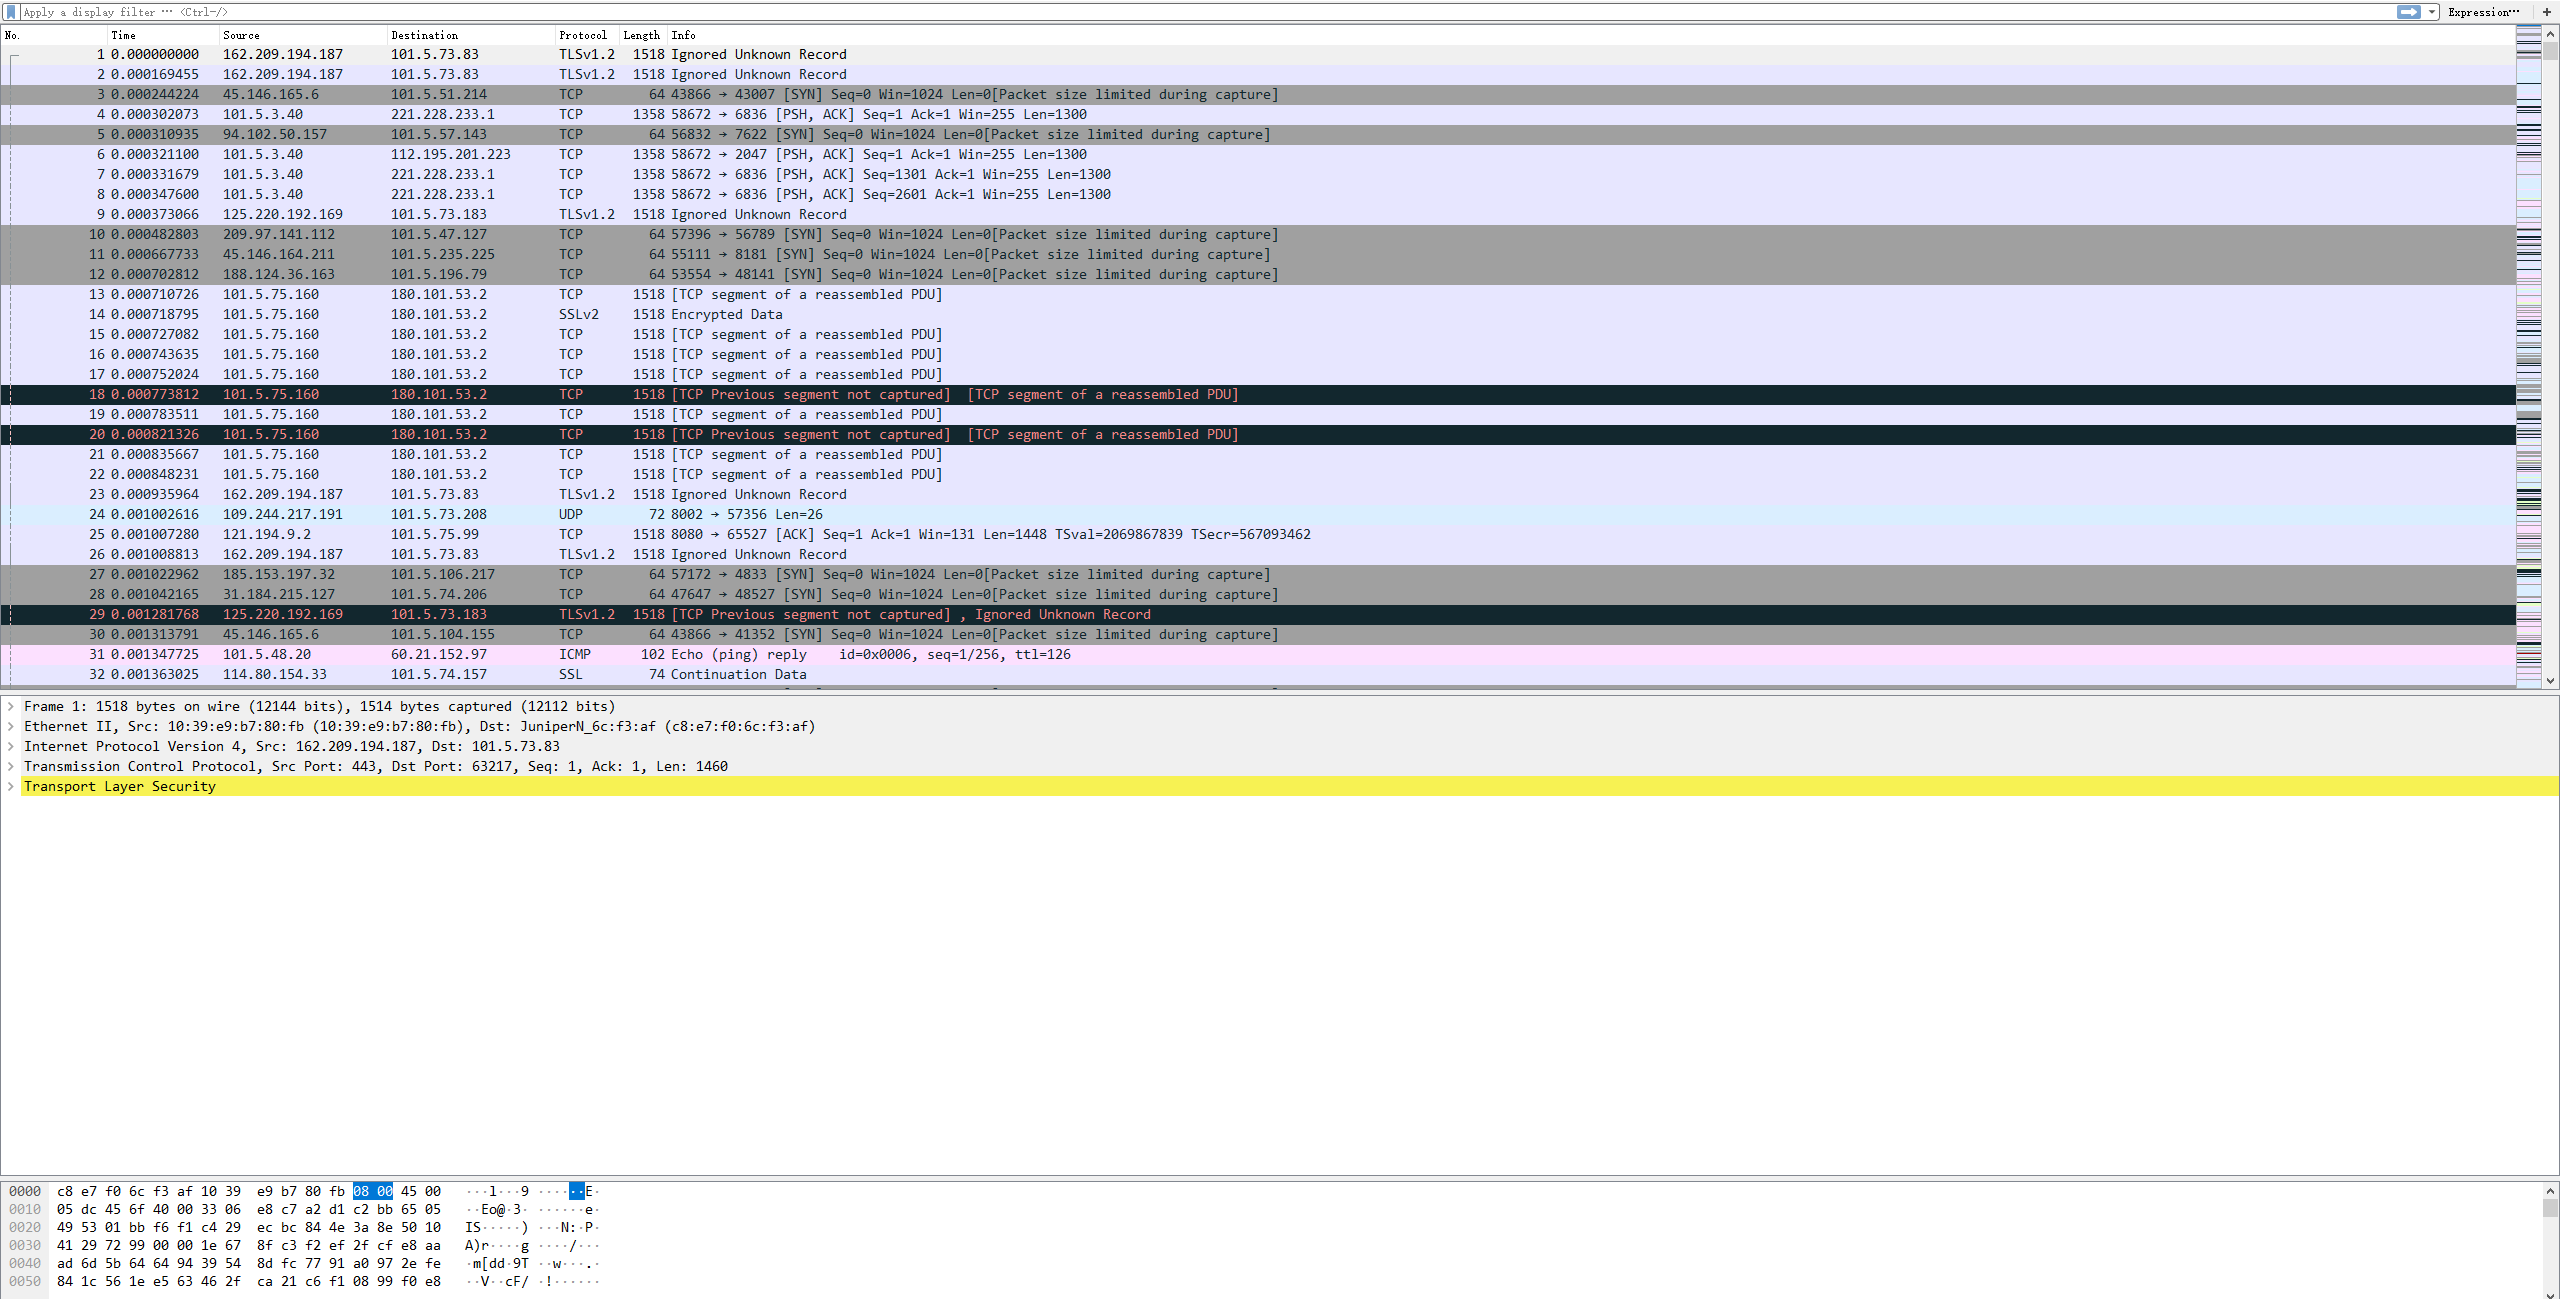
\includegraphics[width=0.6\linewidth]{wireshark流量图.png}
%     \caption{spark分布式运行架构}
%     \label{fig:spark}
%   \end{figure}

\section{系统整体设计}
Spark Streaming是Spark Core为支持流式处理的扩展,具有高容错,高吞吐的特点。Spark Streaming在Spark Core的基础上继续实现StreamingContext(负责管理Spark Streaming程序运行的环境),JobScheduler(负责调度Job任务),JobGenerator(负责生成Job任务),Receiver(负责接收数据)组件。

Spark Streaming内部的基本工作原理如图~\ref{fig:spark工作原理}所示,接收实时输入数据流,然后将数据拆分成多个batch,比如每收集1秒的数据封装为一个batch,然后将每个batch交给Spark的计算引擎进行处理,最后会生产出一个结果数据流,其中的数据,也是由一个一个的batch所组成的。

\begin{figure}
    \centering
    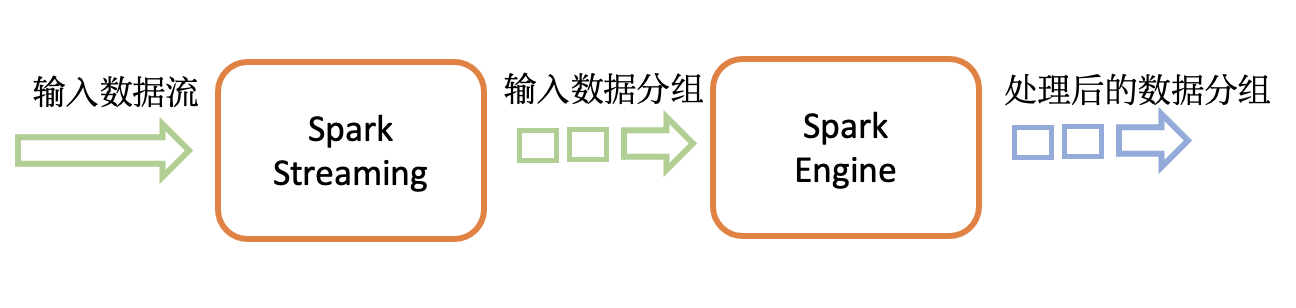
\includegraphics[scale=0.6]{spark工作原理.png}
    % 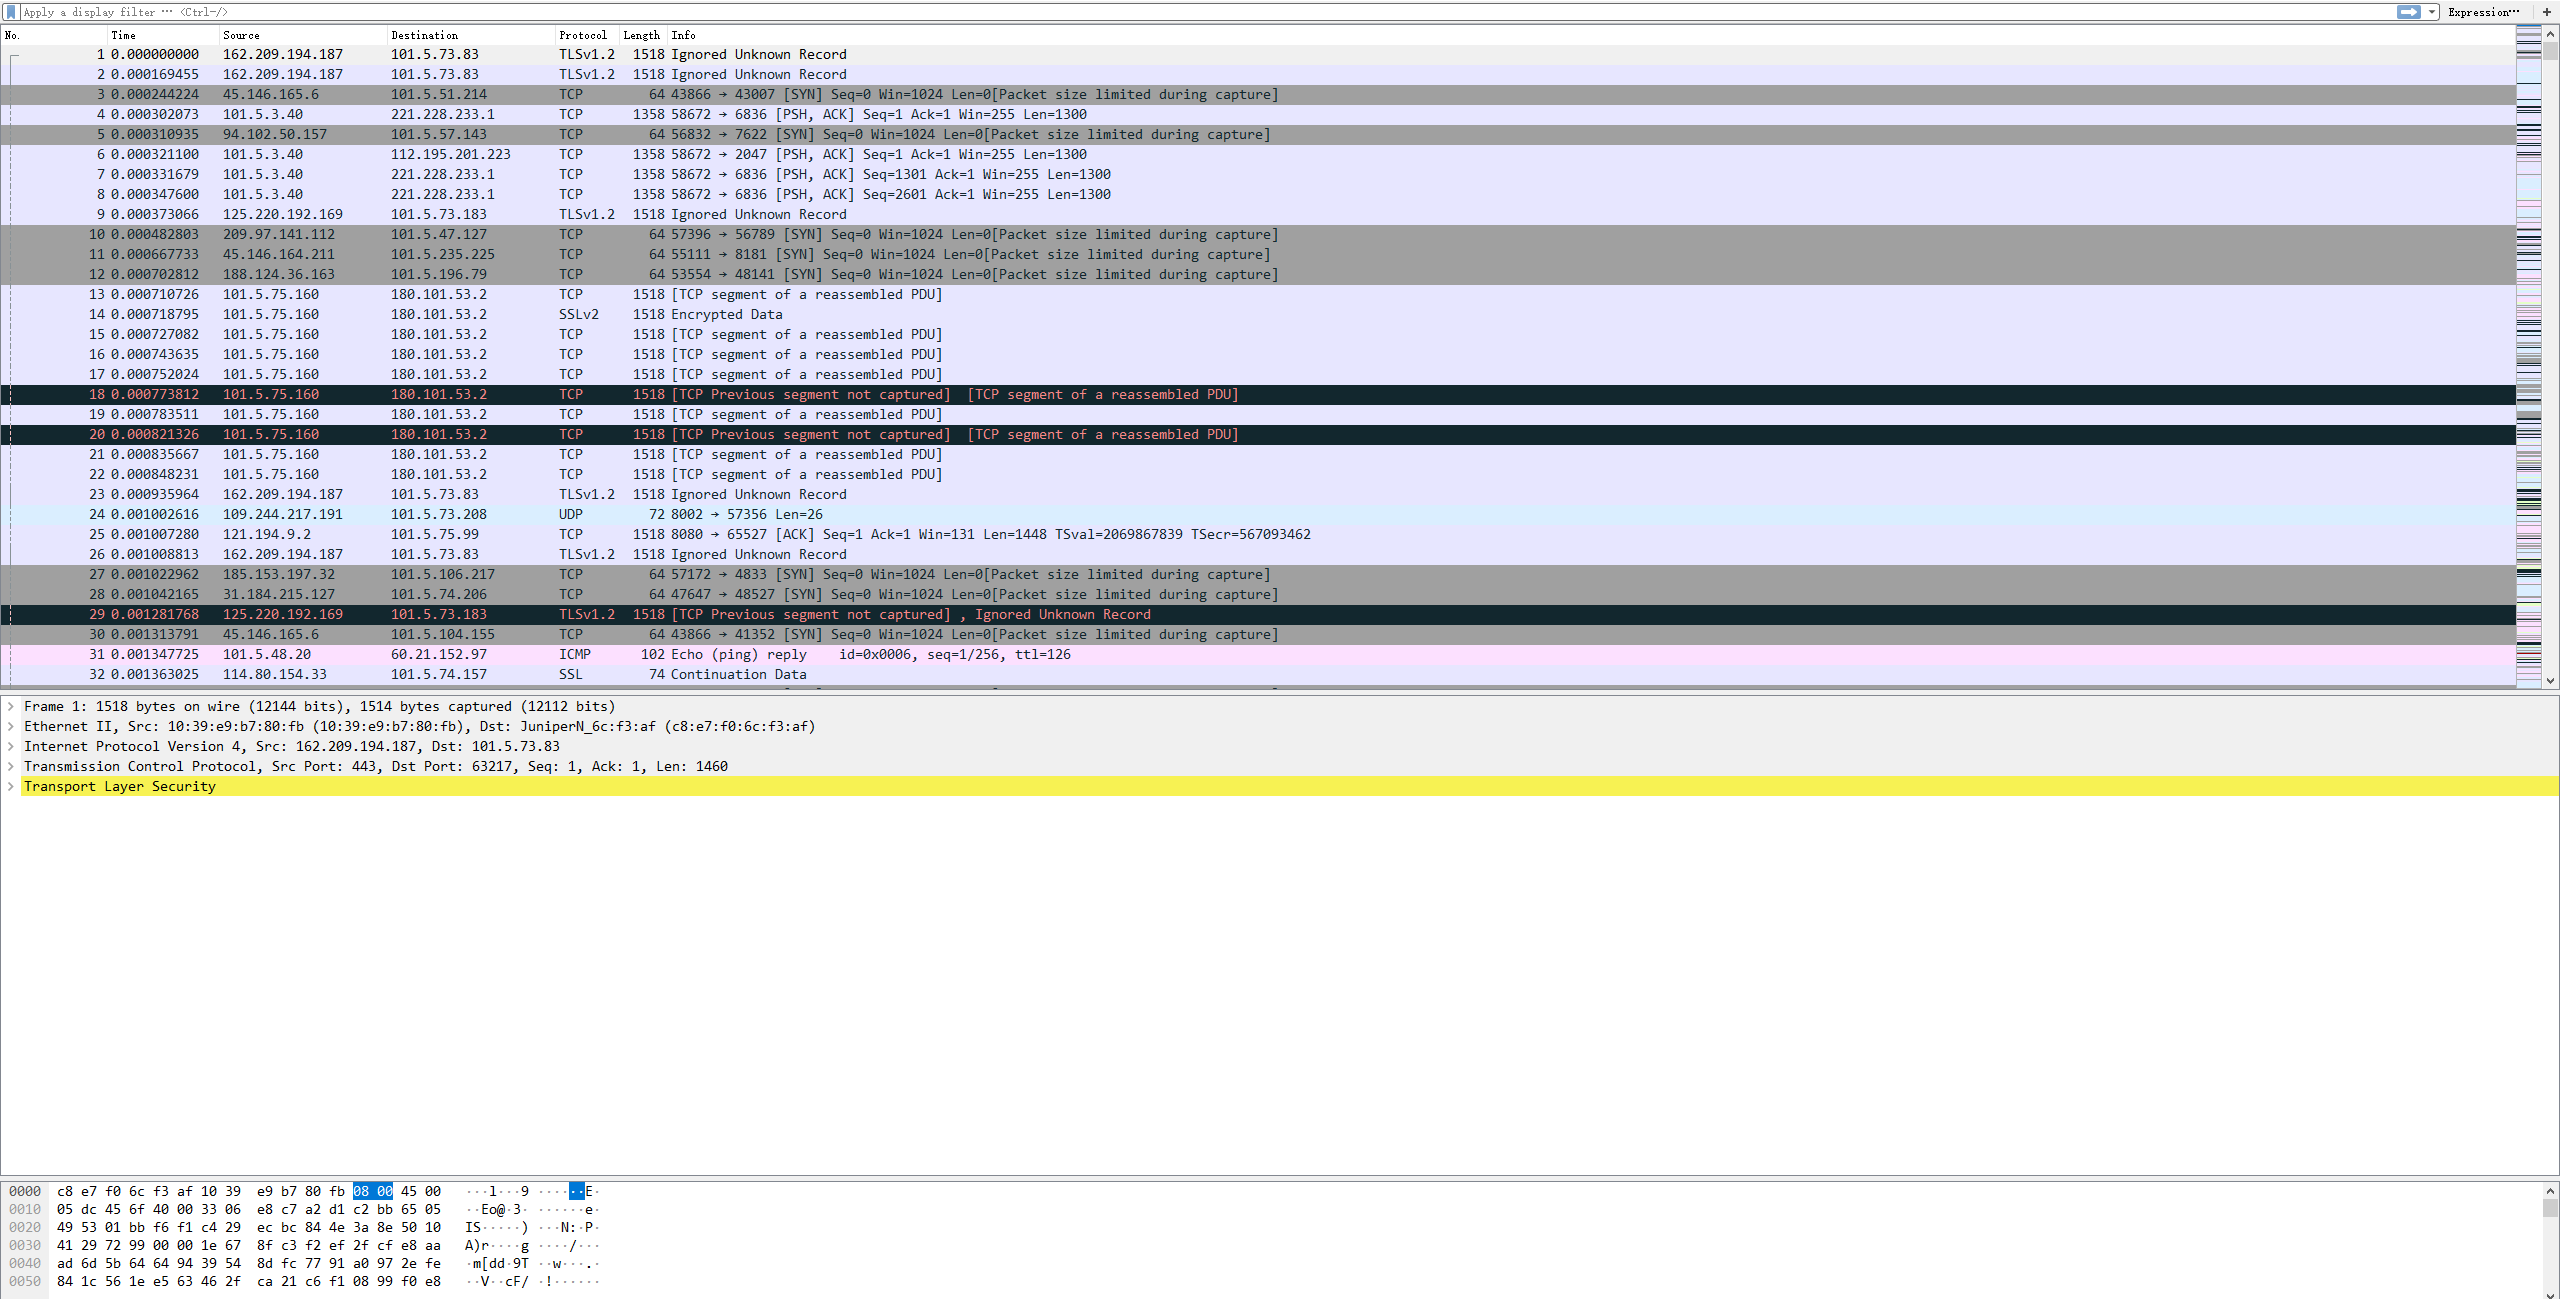
\includegraphics[width=0.6\linewidth]{wireshark流量图.png}
    \caption{spark工作原理}
    \label{fig:spark工作原理}
  \end{figure}

DStream是Spark Streaming中对数据流的一个抽象。DStream以哈希表的方式保存一
系列连续的RDD,哈希表的键是时间,值是RDD。随着时间的推移,DStream中产生新
的RDD,形成一个RDD流,但是由于RDD还是批处理方式,而且往往RDD中的数据量相
对较小,所以SparkStreaming对于数据的处理又称为微批处理。此外DStream和RDD—样,
提供map、foreach、flatMap、transform等算子。

Spark Streaming支持基本数据源和高级数据源,其中基本数据源包括hdfs(hadoop File System)文件源,简单socket源等,高级数据源包括kafka,Flume等。Spark Streaming
在执行的过程可以分成两个阶段,数据准备阶段和数据计算阶段,以下分别介绍。

下图~\ref{fig:spark}展示Spark Streaming接收数据的示意图,其中BlockGenerator,Receiver都是
Spark Streaming实现的组件,blockForPushing是一个阻塞队列。在Spark Streaming数
据准备阶段,首先Receiver从外部数据源接收数据并且将数据写入BlockGenerator的
ArrayBuffer(内存数组)中,该过程会保证数据接收速率始终小于设置的最大速率
maxRate,这个maxRate也可以由Spark的反压模块根据Spark集群的处理速度自行计算。
然后,BlockGenerator包含定时器Timer会定时将ArrayBuffer中的数据生成Block对象(块
对象,其中包含生成的数据),并且将Block对象写入BlockForPushing阻塞队列中,然后
再通知SparkStreaming的Driver程序,将Block对象分配至Block队列。最终,数据在Block
队列中等待Spark Streaming的计算阶段。以上便是Spark Streaming接收数据的全部过程。
\begin{figure}
    \centering
    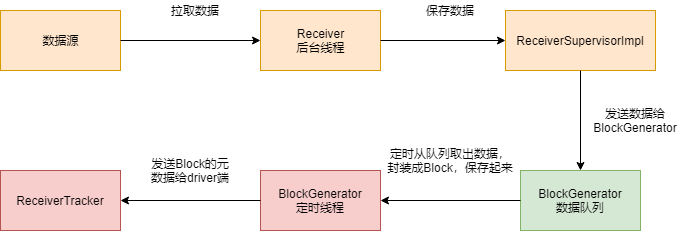
\includegraphics[scale=0.6]{spark数据源.png}
    \caption{Spark数据源}
    \label{fig:spark}
  \end{figure}

  下图~\ref{fig:spark streaming}是Spark Streaming作业的执行流程,具体流程分为以下几步:
  \begin{figure}
    \centering
    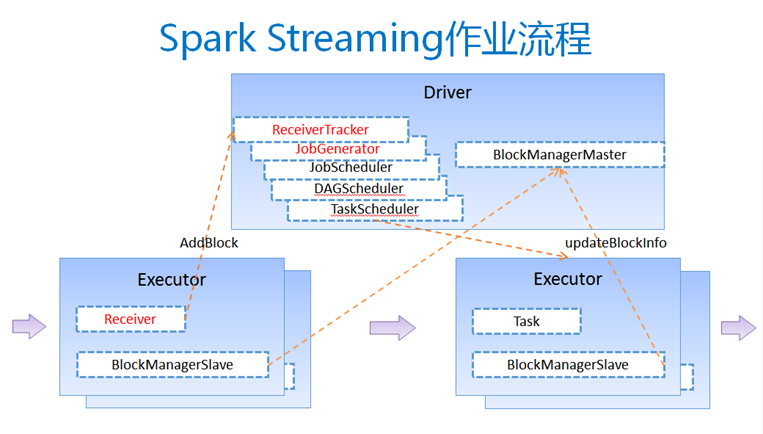
\includegraphics[scale=0.6]{spark执行流程.png}
    \caption{spark streaming执行流程}
    \label{fig:spark streaming}
  \end{figure}
 
  \begin{enumerate}[1.]
      \item  客户端提交作业后启动Driver,Driver是park作业的Master。
      \item 每个作业包含多个Executor,每个Executor以线程的方式运行task,Spark Streaming至少包含一个receiver task。
      \item Receiver接收数据后生成Block,并把BlockId汇报给Driver,然后备份到另外一个Executor上。
      \item ReceiverTracker维护Reciver汇报的BlockId。
      \item Driver定时启动JobGenerator,根据Dstream的关系生成逻辑RDD,然后创建Jobset,交给JobScheduler。
      \item JobScheduler负责调度Jobset,交给DAGScheduler,DAGScheduler根据逻辑RDD,生成相应的Stages,每个stage包含一到多个task。
      \item TaskScheduler负责把task调度到Executor上,并维护task的运行状态。
      \item 当tasks,stages,jobset完成后,单个batch才算完成。
  \end{enumerate}

  运行一个Spark Streaming应用程序,有下面一些步骤

  有管理器的集群-这是任何Spark应用程序都需要的需求,详见部署指南
  将应用程序打为jar包-你必须编译你的应用程序为jar包。如果你用spark-submit启动应用程序,你不需要将Spark和Spark Streaming打包进这个jar包。如果你的应用程序用到了高级源(如kafka,flume),你需要将它们关联的外部artifact以及它们的依赖打包进需要部署的应用程序jar包中。例如,一个应用程序用到了TwitterUtils,那么就需要将spark-streaming-twitter\_2.10以及它的所有依赖打包到应用程序jar中。
  为executors配置足够的内存-因为接收的数据必须存储在内存中,executors必须配置足够的内存用来保存接收的数据。注意,如果你正在做10分钟的窗口操作,系统的内存要至少能保存10分钟的数据。所以,应用程序的内存需求依赖于使用它的操作。
  配置checkpointing-如果stream应用程序需要checkpointing,然后一个与Hadoop API兼容的容错存储目录必须配置为检查点的目录,流应用程序将checkpoint信息写入该目录用于错误恢复。
  配置应用程序driver的自动重启-为了自动从driver故障中恢复,运行流应用程序的部署设施必须能监控driver进程,如果失败了能够重启它。不同的集群管理器,有不同的工具得到该功能
  
  Spark Standalone:一个Spark应用程序driver可以提交到Spark独立集群运行,也就是说driver运行在一个worker节点上。进一步来看,独立的集群管理器能够被指示用来监控driver,并且在driver失败(或者是由于非零的退出代码如exit(1),或者由于运行driver的节点的故障)的情况下重启driver。
  YARN:YARN为自动重启应用程序提供了类似的机制。
  Mesos: Mesos可以用Marathon提供该功能
  
  配置write ahead logs-在Spark 1.2中,为了获得极强的容错保证,我们引入了一个新的实验性的特性-预写日志(write ahead logs)。如果该特性开启,从receiver获取的所有数据会将预写日志写入配置的checkpoint目录。这可以防止driver故障丢失数据,从而保证零数据丢失。这个功能可以通过设置配置参数spark.streaming.receiver.writeAheadLogs.enable为true来开启。然而,这些较强的语义可能以receiver的接收吞吐量为代价。这可以通过并行运行多个receiver增加吞吐量来解决。另外,当预写日志开启时,Spark中的复制数据的功能推荐不用,因为该日志已经存储在了一个副本在存储系统中。可以通过设置输入DStream的存储级别为StorageLevel.MEMORY\_AND\_DISK\_SER获得该功能。

安装环境介绍(待补充):
本文将 Spark 部署在安装有 ubuntu16.04 系统的 VirtualBox 虚拟机中。

搭建 Spark 集群,需要准备以下文件及环境:
jdk-8u211-linux-x64.tar.gz
spark-2.4.3-bin-hadoop2.7.tgz
3 个独立的 ubuntu16.04 虚拟机系统,机器集群规划如下:

\section{流式数据特征抽取}
Spark Streaming 支持 Scala、Java 和 Python,本文中使用Python提交任务。使用第三章中的特征提取方法,
输入为由kafka传入的流量数据,提取的结果都是传输层的一些统计信息,以一个TCP流或一个UDP流为一个单位。TCP流以FIN标志为结束,UDP以设置的flowtimeout时间为限制,超过时间就判为结束。在一个TCP流中有很多个数据包,先三次握手而后传输信息再四次挥手。统计一个流中的统计信息作为提取的特征。且统计的特征都分前后向,规定由源地址到目的地址为正向,目的地址到源地址为反向,例如某条TCP流的源ip地址为192.168.31.100,源端口号为174,目的ip地址为183.232.231.174,目的端口号为443,则为该流构建一个标志叫Flow ID:192.168.31.100-183.232.231.174-46927-443-6,由源地址、目的地址、源端口、目的端口、协议号组成。
流量特征提取的整体流程图如下:

\begin{figure}
    \centering
    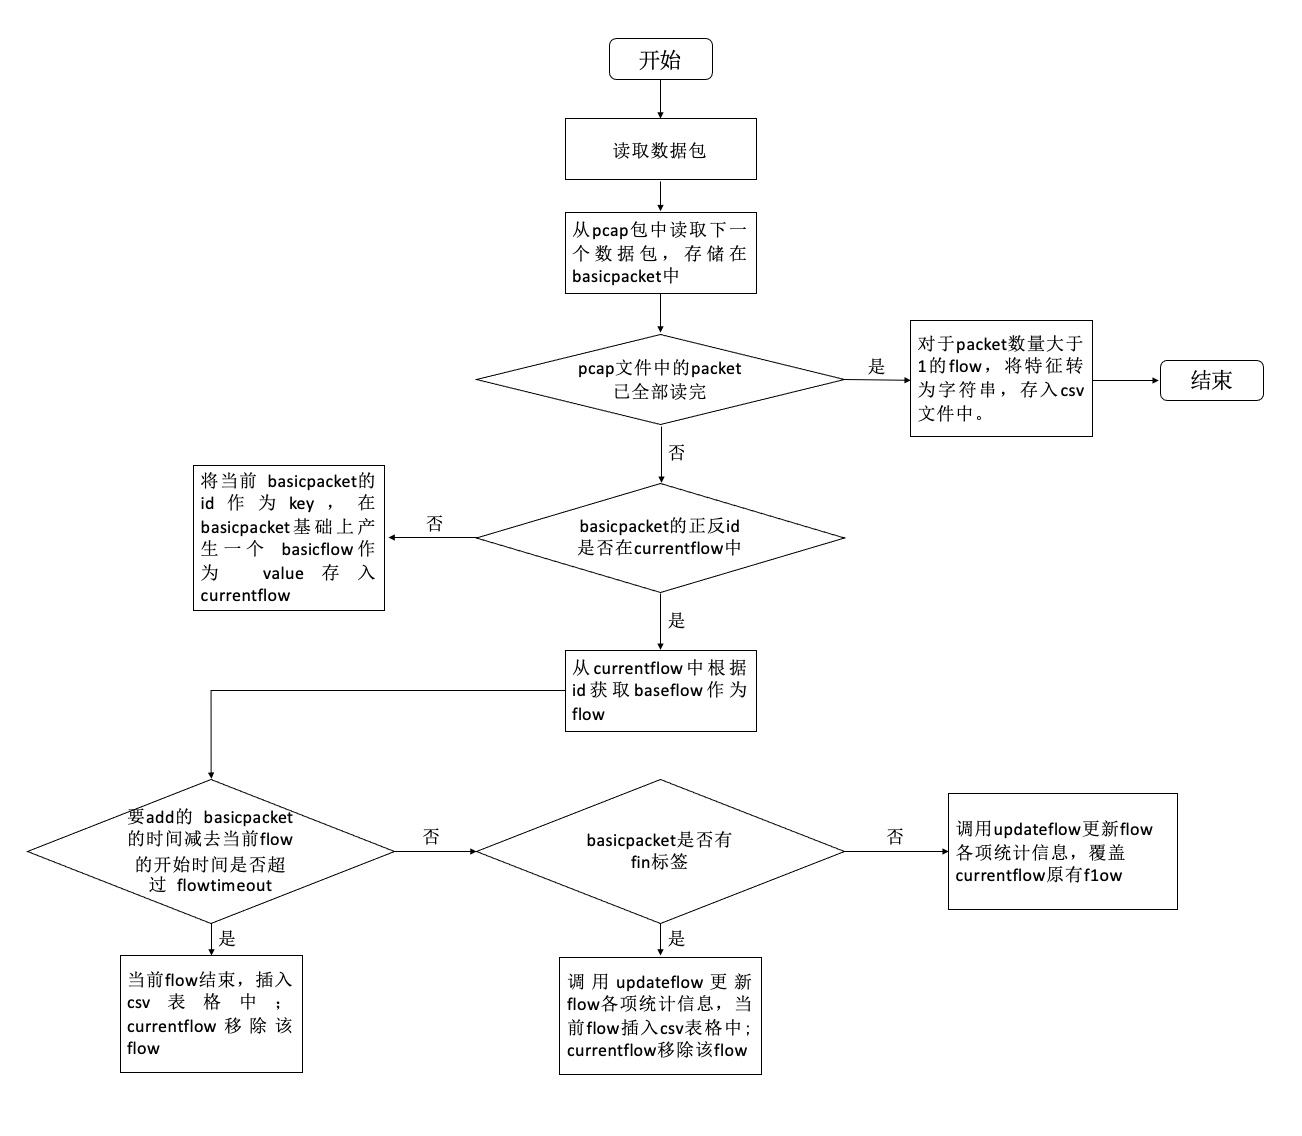
\includegraphics[scale=0.3]{特征提取.jpg}
    \caption{特征提取}
    \label{fig:特征提取}
  \end{figure}

从pcap文件中逐个读取packet,将每个数据包添加到对应的流中在currentFlows存储当前还未结束得所有TCP、UDP流。在添加的过程中不断地更新每个流的统计特征,最终将统计特征写入csv文件。判断新加入的数据包是否属于当前所有未结束的流,如果属于当前流则判断正向还是反向,之后判断时间是否超时、不超时则判断是否含有FIN标志,如果两者都不满足,则声明一个BasicFlow对象,根据id从currentFlows中拿到与当前数据包对应的流,调用addPacket将该数据包加入到对应流中。如果前面判断不在当前所有未结束的流中,则直接创建一个新得流,里面只含当前数据包,存入到currentFlows中。如果属于当前某个未结束的流,且超时或存在FIN标志,则说明当前flow结束,超时则从currentFlows中移除对应流,新建flow存入currentFlows中,含FIN标志则直接从currentFlows中移除对应流。结束的flow直接调用onFlowGenerated函数将流打印存储起来。

使用该方法得到的csv文件如下所示:
\begin{figure}
    \centering
    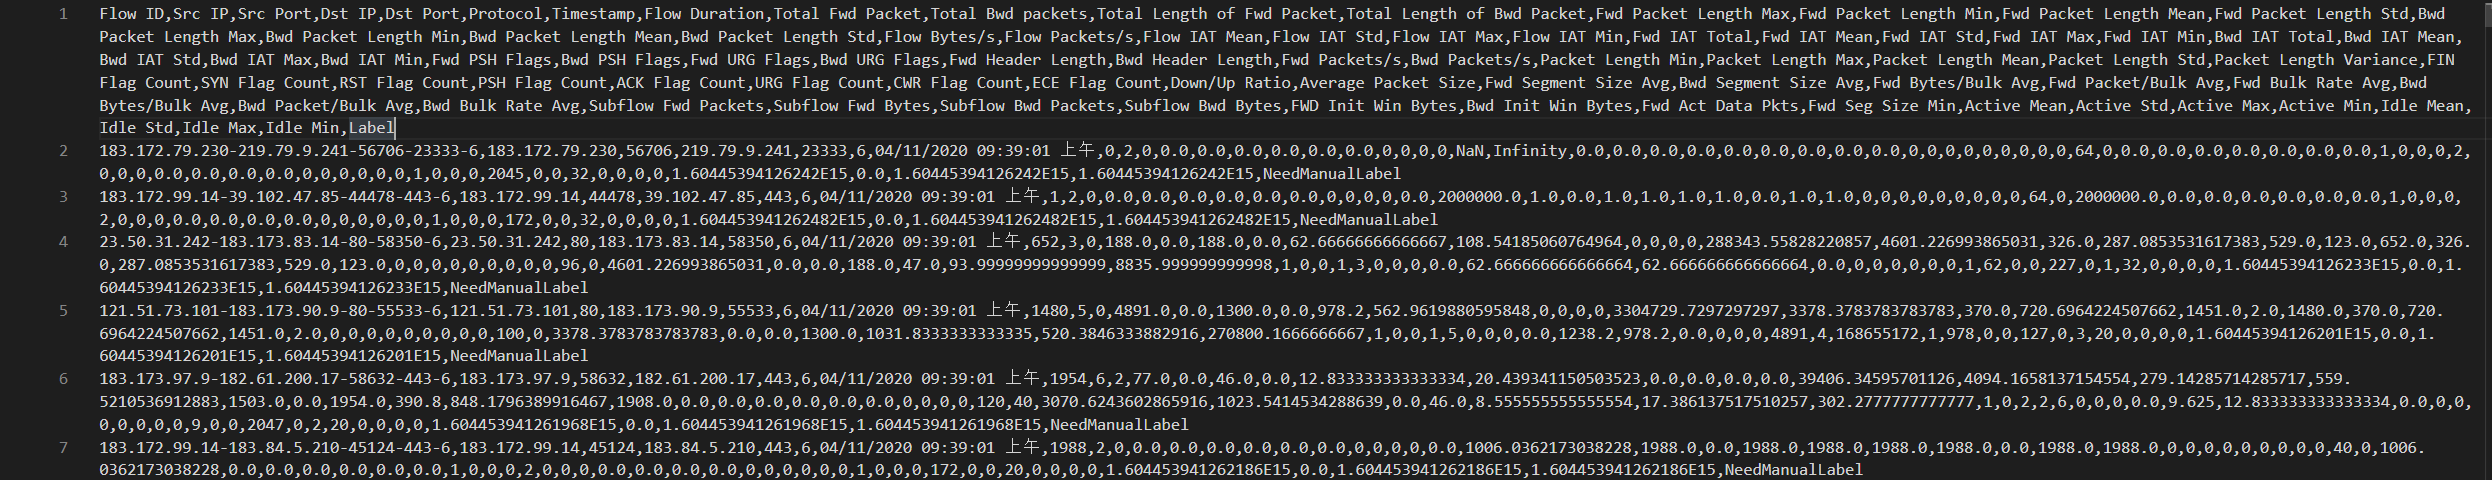
\includegraphics[scale=0.2]{特征文件.png}
    \caption{特征文件}
    \label{fig:特征文件}
  \end{figure}


\section{模型训练模块的设计与实现}
补充一些图
\begin{figure}
  \centering
  
\includegraphics[width=0.6\linewidth]{example-image-a.pdf}
  \caption{Example figure in appendix}
  \label{fig:appendix-survey-figure}
\end{figure}
\section{预测输出模块}
\section{系统结果展示与分析}
本章在第二章技术分析和介绍的基础上,先后阐述异常流量检测系统的需求分析、
本文系统总体架构的设计、算法模型的设计方案,最后根据系统的总系架构和算法模型
提出本文系统五大模块的设计方案。
3.1需求分析
3.1.1功能需求分析
根据项目背景,本文设计的系统功能需求为:
(1)能够通过JnetPcap技术采集主机流量特征,采集pcap类型文件中的保存的流量特
征。
(2)能够将采集端的采集特征在后台收集端集中,过滤,写入kafka。
(3)能够对流量预测,本文将流量分成4等级,等级越高,是异常流量的可能性越大。
(4)能够对预测的结果进行良好的展示。
(5)预测模型具有一定效果。
3.1.2系统需求分析
(1)可扩展:随着后期需求的变化与增长,所以在开发过程需要考虑如何应付这些后
期变化。针对本系统,需要考虑采集模块支持Windows、Linux系统,需要考虑预测模块
中模型的更新和替换问题。
(2)健壮性:在流式处理的过程中,有可能其中一个模块偶尔发生错误,不能让这种
错误影响到整体系统运行,但是需要对这种错误进行记录。
(3)配置分离:系统的某些属性需要以配置文件的形式分离出来,方便以后对系统的
管理控制。
3.2系统总体设计
3.2.1异常流量预测系统总体架构设计
本系统属于流式系统,采集模块获取数据包流量的特征,并且实时对流量进行预测,
最后以报表的形式展示出来。结合需求和相关技术的分析,本文系统总体设计如图所
示,下面分别对各个模块的功能进行介绍。

3.2.2异常流量预测系统运行流程简介
在系统环境已经部署好的情况下,结合异常流量的总体架构设计,该系统运行的整
体流程如图3-2所示,图中编号代表这个模块运行的步骤。
% (1)训练离线模型。离线模型训练需要脱离整个数据流运行,本系统主要具有两个模
% 型,分另丨J是KMeans
% _
% RandomForest
% _
% Model和Streaming
% _
% KJVleans
% _
% Model,其中
% KMeans
% _
% RandomForest
% _
% Model基于K-Means算法和RandomForest算法实现,是监督模
% 型,需要标注数据,预测效果好;Streaming
% +
% KMeans
% +
% Modd是无监督的机器学习模型,
% 18
% 不需要标注数据,但是需要提供初始化参数,该模型预测效果不如
% KMeans
% —
% RandomForest
% —
% Model〇
(2)开启后台收集模块,收集端应该先于采集端运行,不然会导致采集端发送的数据
丢失。
(3)开启采集模块,采集并发送数据。
(4)向Spark集群提交预测模块任务,从kafka中源源不断的读取数据,并且将预测后
的结果写入一个新的kafka topic。
(4)开启报表模块展示预测结果。